\documentclass[12pt,a4paper]{article}

\usepackage{fontspec}
\setmainfont{Tinos}
\setsansfont{Arimo}
\setmonofont{DejaVu Sans Mono}
\usepackage[russian]{babel}
\usepackage{geometry}
\geometry{left=38mm,right=25mm,top=38mm,bottom=25mm}
\usepackage{setspace}
\onehalfspacing
\usepackage{indentfirst}
\setlength{\parindent}{1.25cm}
\setlength{\emergencystretch}{3em}

\usepackage{xcolor}
\usepackage{listings}
\usepackage{booktabs}
\usepackage{array}
\usepackage{graphicx}
\usepackage{float}
\usepackage{caption}
\usepackage{titlesec}
\usepackage{needspace}
\usepackage{tikz}
\usetikzlibrary{arrows.meta,positioning}
\usepackage{xurl}
\usepackage{hyperref}
\hypersetup{colorlinks=true,linkcolor=black,urlcolor=blue}
\usepackage{fancyhdr}
\pagestyle{fancy}
\fancyhf{}
\fancyfoot[C]{\thepage}
\renewcommand{\headrulewidth}{0pt}

\newcommand{\studentName}{Пантюхин Никита Олегович}
\newcommand{\studentGroup}{М8О-201БВ-25}
\newcommand{\checkerName}{Миронов Евгений Сергеевич}
\newcommand{\repoUrl}{https://github.com/nikitapantyukhin/operating-systems-and-computer-architecture-y2-s3/tree/main/lab2}

\definecolor{codebg}{RGB}{247,247,247}
\definecolor{codeframe}{RGB}{205,205,205}
\definecolor{codecomment}{RGB}{70,110,70}
\definecolor{codekeyword}{RGB}{30,70,150}
\definecolor{headingone}{HTML}{1F3864}
\definecolor{headingtwo}{HTML}{2E5FA3}
\renewcommand{\lstlistingname}{Листинг}
\DeclareCaptionLabelSeparator{reportdash}{~---~}
\captionsetup[lstlisting]{labelsep=reportdash}

\titleformat{\section}
  {\color{headingone}\bfseries\fontsize{14}{17}\selectfont}
  {\thesection.}{0.5em}{}
\titleformat{\subsection}
  {\color{headingtwo}\bfseries\fontsize{13}{16}\selectfont}
  {\thesubsection.}{0.5em}{}
\titlespacing*{\section}{0pt}{18pt}{9pt}
\titlespacing*{\subsection}{0pt}{12pt}{6pt}

\lstdefinestyle{cstyle}{
  language=C,
  basicstyle=\ttfamily\footnotesize,
  keywordstyle=\color{codekeyword}\bfseries,
  commentstyle=\color{codecomment},
  backgroundcolor=\color{codebg},
  frame=single,
  rulecolor=\color{codeframe},
  breaklines=true,
  breakatwhitespace=false,
  showstringspaces=false,
  tabsize=4,
  columns=fullflexible,
  keepspaces=true,
  captionpos=b,
  aboveskip=0.7em,
  belowskip=0.9em
}

\lstdefinestyle{terminal}{
  basicstyle=\ttfamily\footnotesize,
  backgroundcolor=\color{codebg},
  frame=single,
  rulecolor=\color{codeframe},
  breaklines=true,
  breakatwhitespace=false,
  showstringspaces=false,
  columns=fullflexible,
  keepspaces=true,
  captionpos=b,
  aboveskip=0.7em,
  belowskip=0.9em
}

\begin{document}

\begin{titlepage}
\thispagestyle{empty}
\begin{center}
{\fontsize{10}{12}\selectfont\bfseries
МИНИСТЕРСТВО НАУКИ И ВЫСШЕГО ОБРАЗОВАНИЯ\\
РОССИЙСКОЙ ФЕДЕРАЦИИ}\\[0.2cm]
{\fontsize{10}{12}\selectfont
Федеральное государственное автономное образовательное учреждение высшего образования\\
\textbf{«Московский авиационный институт\\
(национальный исследовательский университет)»}}

\vspace{2.2cm}
{\fontsize{16}{19}\selectfont\bfseries ОТЧЁТ ПО ЛАБОРАТОРНОЙ РАБОТЕ}\\[0.15cm]
{\fontsize{16}{19}\selectfont\bfseries № 2}

\vspace{0.9cm}
\textbf{Дисциплина:}\\[0.15cm]
Операционные системы и архитектура компьютера

\vspace{0.7cm}
\textbf{Тема:}\\[0.15cm]
Управление процессами и обмен данными посредством каналов

\vspace{2.0cm}
\begin{flushright}
\textbf{Выполнил:}\\[0.15cm]
студент группы \studentGroup\\[0.1cm]
\studentName\\[0.6cm]
\textbf{Проверил:}\\[0.15cm]
Преподаватель\\[0.1cm]
\checkerName
\end{flushright}

\vfill
Москва, 2026 г.
\end{center}
\end{titlepage}

\setcounter{page}{2}
\tableofcontents
\newpage

\section{Цель работы}

Цель работы --- на практике изучить взаимодействие процессов в Linux: создание дочернего процесса с помощью \texttt{fork()}, передачу данных через неименованный канал \texttt{pipe}, перенаправление стандартного ввода функцией \texttt{dup2()}, запуск отдельной программы через \texttt{exec} и ожидание её завершения с помощью \texttt{waitpid()}.

\section{Краткое описание архитектуры решения}

Лабораторная работа состоит из двух отдельных программ: \texttt{parent} и \texttt{child}. Программа \texttt{parent} запрашивает имя выходного файла, создаёт один неименованный канал и вызывает \texttt{fork()}. В дочерней ветке закрывается write-end канала, а read-end перенаправляется в \texttt{STDIN\_FILENO} с помощью \texttt{dup2()}. После этого выполняется \texttt{execl("./child", ...)}, который заменяет программу дочернего процесса программой \texttt{child}.

Родительский процесс закрывает read-end канала, читает строки чисел с клавиатуры и передаёт их через write-end. Программа \texttt{child} получает эти строки через обычный \texttt{stdin}, проверяет целые числа, вычисляет сумму каждой строки и записывает результат в выбранный файл. После EOF родитель закрывает канал и ожидает завершения дочернего процесса через \texttt{waitpid()}.

Программы запускаются из каталога \texttt{build/}, поэтому файлы \texttt{parent} и \texttt{child} находятся рядом. Сигнал \texttt{SIGPIPE} игнорируется простым вызовом \texttt{signal()}, чтобы при преждевременном завершении \texttt{child} родитель мог получить и обработать ошибку записи в канал.

\subsection{Схема взаимодействия компонентов}

На рисунке показано направление передачи данных между пользователем, родительским процессом, каналом, дочерним процессом и выходным файлом.

\begin{figure}[H]
\centering
\begin{tikzpicture}[
  node distance=0.75cm,
  block/.style={draw,rounded corners,minimum width=5.4cm,minimum height=0.8cm,align=center},
  arrow/.style={-{Latex[length=2.5mm]},thick},
  label/.style={fill=white,inner sep=1.5pt,font=\small}
]
\node[block] (terminal) {stdin терминала};
\node[block,below=of terminal] (parent) {parent};
\node[block,below=of parent] (pipe) {неименованный канал pipe};
\node[block,below=of pipe] (child) {child};
\node[block,below=of child] (file) {выходной файл};
\draw[arrow] (terminal) -- node[label,right]{имя файла и строки чисел} (parent);
\draw[arrow] (parent) -- node[label,right]{write-end} (pipe);
\draw[arrow] (pipe) -- node[label,right]{read-end $\rightarrow$ dup2 $\rightarrow$ stdin} (child);
\draw[arrow] (child) -- node[label,right]{суммы строк} (file);
\end{tikzpicture}
\caption*{Рисунок~--- Схема взаимодействия компонентов программы}
\end{figure}

Канал создаётся до \texttt{fork()}, поэтому оба процесса получают его файловые дескрипторы. Каждый процесс закрывает неиспользуемый конец канала. Благодаря \texttt{dup2()} программа \texttt{child} может читать данные через стандартный ввод и не зависит от деталей передачи данных в \texttt{parent}.

\section{Листинг ключевых фрагментов кода}

Сначала родитель создаёт канал и дочерний процесс. При ошибках системных вызовов программа выводит сообщение и завершает работу.

\begin{lstlisting}[style=cstyle,caption={Создание канала и дочернего процесса},label={lst:pipe-fork}]
int pipefd[2];

if (pipe(pipefd) == -1) {
    perror("pipe");
    /* освобождение ресурсов */
    return 1;
}

pid_t pid = fork();

if (pid == -1) {
    perror("fork");
    /* освобождение ресурсов */
    return 1;
}
\end{lstlisting}

В дочерней ветке write-end закрывается, read-end становится стандартным вводом, после чего запускается отдельная программа \texttt{child}.

\begin{lstlisting}[style=cstyle,caption={Перенаправление stdin и запуск программы child},label={lst:dup2-exec}]
if (pid == 0) {
    close(pipefd[1]);

    if (dup2(pipefd[0], STDIN_FILENO) == -1) {
        perror("dup2");
        close(pipefd[0]);
        free(filename);
        _exit(1);
    }

    close(pipefd[0]);
    execl("./child", "child", filename, NULL);
    perror("execl");
    free(filename);
    _exit(1);
}
\end{lstlisting}

Родитель читает строки до EOF и передаёт каждую строку целиком через канал. Функция \texttt{write\_all()} учитывает возможность частичной записи.

\begin{lstlisting}[style=cstyle,caption={Передача пользовательских строк через pipe},label={lst:parent-write}]
while ((line_length = getline(&line, &line_size, stdin)) != -1) {
    if (write_all(pipefd[1], line, (size_t)line_length) == -1) {
        parent_error = 1;
        break;
    }
}

free(line);
close(pipefd[1]);
\end{lstlisting}

\Needspace{0.70\textheight}
Программа \texttt{child} читает строку из перенаправленного \texttt{stdin}, разбирает её на целые числа и записывает вычисленную сумму в файл.

\begin{lstlisting}[style=cstyle,caption={Чтение чисел, вычисление суммы и запись результата},label={lst:child-sum}]
while (getline(&line, &line_size, stdin) != -1) {
    long long sum = 0;
    char *token = strtok(line, " \t\r\n");
    while (token != NULL) {
        errno = 0;
        char *end = NULL;
        long number = strtol(token, &end, 10);
        if (end == token || *end != '\0' || errno == ERANGE ||
            number < INT_MIN || number > INT_MAX) {
            fprintf(stderr, "Invalid number: %s\n", token);
            return cleanup_on_error(line, file_fd);
        }
        sum += number;
        token = strtok(NULL, " \t\r\n");
    }
    char result[64];
    int result_length = snprintf(result, sizeof(result), "%lld\n", sum);
    if (write_all(file_fd, result, (size_t)result_length) == -1) {
        return cleanup_on_error(line, file_fd);
    }
}
\end{lstlisting}

После закрытия канала родитель ожидает дочерний процесс и проверяет его статус. Это не позволяет завершившемуся дочернему процессу остаться в состоянии zombie.

\begin{lstlisting}[style=cstyle,caption={Ожидание и проверка завершения child},label={lst:waitpid}]
int status;
if (waitpid(pid, &status, 0) == -1) {
    perror("waitpid");
    return 1;
}
if (check_child_status(status) == -1) {
    parent_error = 1;
}
\end{lstlisting}

Полный исходный код доступен в
\href{\repoUrl}{GitHub-репозитории лабораторной работы № 2}.

\clearpage
\section{Результаты работы}

Проект был собран с помощью CMake без ошибок и предупреждений. В успешном сценарии программа получила несколько строк целых чисел и записала сумму каждой строки в файл \texttt{result\_file.txt}.

\begin{table}[H]
\centering
\renewcommand{\arraystretch}{1.25}
\begin{tabular}{>{\ttfamily}l >{\ttfamily}r}
\toprule
\normalfont\textbf{Введённая строка} & \normalfont\textbf{Результат} \\
\midrule
2 5 6 7 10 3 & 33 \\
3 9 93939 930 3434 & 98315 \\
1 22 3 & 26 \\
453 34 35 78 & 600 \\
34 7 6 9 53 & 109 \\
\bottomrule
\end{tabular}
\caption*{Таблица~--- Результаты вычисления сумм}
\end{table}

После завершения ввода через EOF родитель закрыл write-end канала, дочерний процесс закончил чтение и корректно завершился. Содержимое выходного файла совпало с рассчитанными суммами.

\subsection{Консольный вывод или логи}

В консоли выводятся PID родительского и дочернего процессов. Это позволяет увидеть, что \texttt{parent} и \texttt{child} работают как два разных процесса.

\begin{lstlisting}[style=terminal,caption={Пример успешного запуска программы},label={lst:console-run}]
$ ./parent
Enter filename: result_file.txt
Parent PID: 317763, Child PID: 318229
Enter numbers line by line. Press Ctrl+D to finish.
Child PID: 318229, Parent PID: 317763
2 5 6 7 10 3
43 8598 98 9485 9459 89485 94898 5948 98984
3 9 93939 930 3434
1 22 3
453 34 35 78
34 7 6 9 53
^D
\end{lstlisting}

\noindent\begin{minipage}{\linewidth}
После завершения программы файл содержит по одной сумме для каждой введённой строки.

\begin{lstlisting}[style=terminal,caption={Проверка содержимого выходного файла},label={lst:result-file}]
$ cat result_file.txt
33
316998
98315
26
600
109
\end{lstlisting}
\end{minipage}

Для проверки системных вызовов программа запускалась из каталога \texttt{build/} под управлением \texttt{strace}. В отчёт включён только фрагмент, относящийся к взаимодействию процессов.

\begin{lstlisting}[style=terminal,caption={Ключевые системные вызовы из трассировки strace},label={lst:strace}]
322069 execve("./parent", ["./parent"], ...) = 0
322069 pipe2([3, 4], 0) = 0
322069 clone(..., SIGCHLD, ...) = 322296
322069 close(3) = 0
322296 close(4) = 0
322296 dup2(3, 0) = 0
322296 close(3) = 0
322296 execve("./child", ["child", "result_file.txt"], ...) = 0
322069 write(4, "2 5 6 7 10 3\n", 17) = 17
322296 write(3, "33\n", 3) = 3
322069 close(4) = 0
322069 wait4(322296, ..., 0, NULL) = 322296
\end{lstlisting}

Трассировка показывает создание канала и второго процесса, перенаправление файлового дескриптора, запуск программы \texttt{child}, передачу строки через канал и ожидание завершения. В Linux библиотечным вызовам \texttt{pipe()}, \texttt{fork()}, \texttt{execl()} и \texttt{waitpid()} в данном запуске соответствуют системные вызовы \texttt{pipe2()}, \texttt{clone()}, \texttt{execve()} и \texttt{wait4()}.

\subsection{Скриншоты результатов}

\begin{figure}[H]
\centering
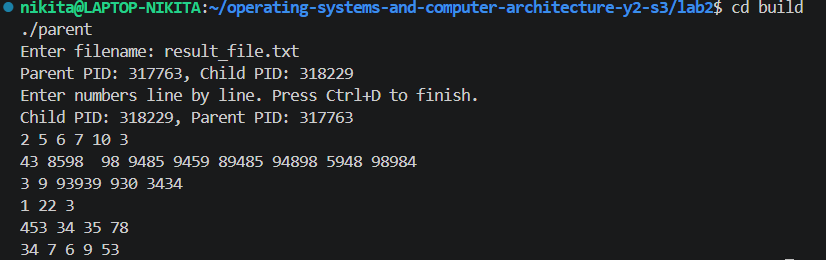
\includegraphics[width=\linewidth,keepaspectratio]{images/success_run.png}
\caption*{Рисунок~--- Успешный запуск родительского и дочернего процессов}
\end{figure}

\begin{figure}[H]
\centering
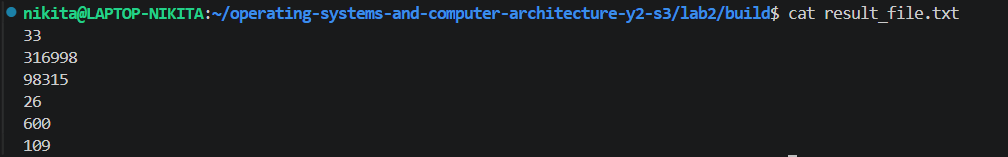
\includegraphics[width=\linewidth,keepaspectratio]{images/result_file.png}
\caption*{Рисунок~--- Результаты вычисления сумм}
\end{figure}

\begin{figure}[H]
\centering
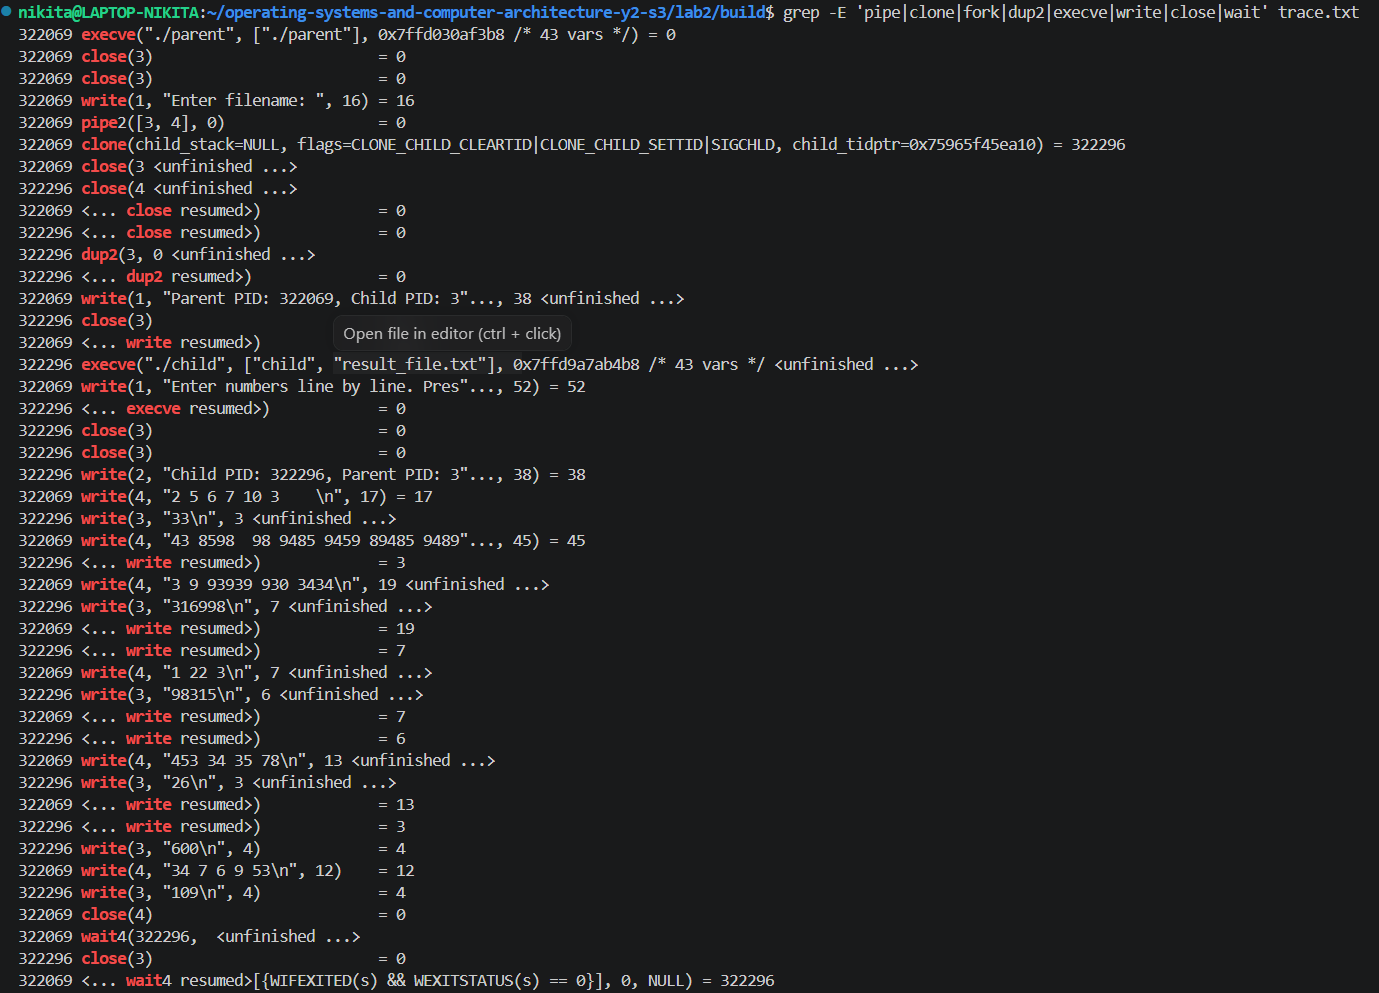
\includegraphics[width=\linewidth,height=0.72\textheight,keepaspectratio]{images/strace.png}
\caption*{Рисунок~--- Системные вызовы при взаимодействии процессов}
\end{figure}

\clearpage
\section{Выводы}

После выполнения этой лабораторной я лучше понял, как в Linux взаимодействуют родительский и дочерний процессы и как данные передаются между ними через \texttt{pipe}. На практике я разобрался, как вместе используются \texttt{fork()}, \texttt{dup2()}, \texttt{exec()} и \texttt{waitpid()}, а также зачем закрывать неиспользуемые концы канала. С помощью \texttt{strace} я увидел системные вызовы, которые реально выполняются при работе программы. Благодаря этому тема процессов и межпроцессного взаимодействия стала для меня намного понятнее.

\end{document}
